\subsection{Features of \Tool{} IDE plugin}

\begin{figure*}
\centering
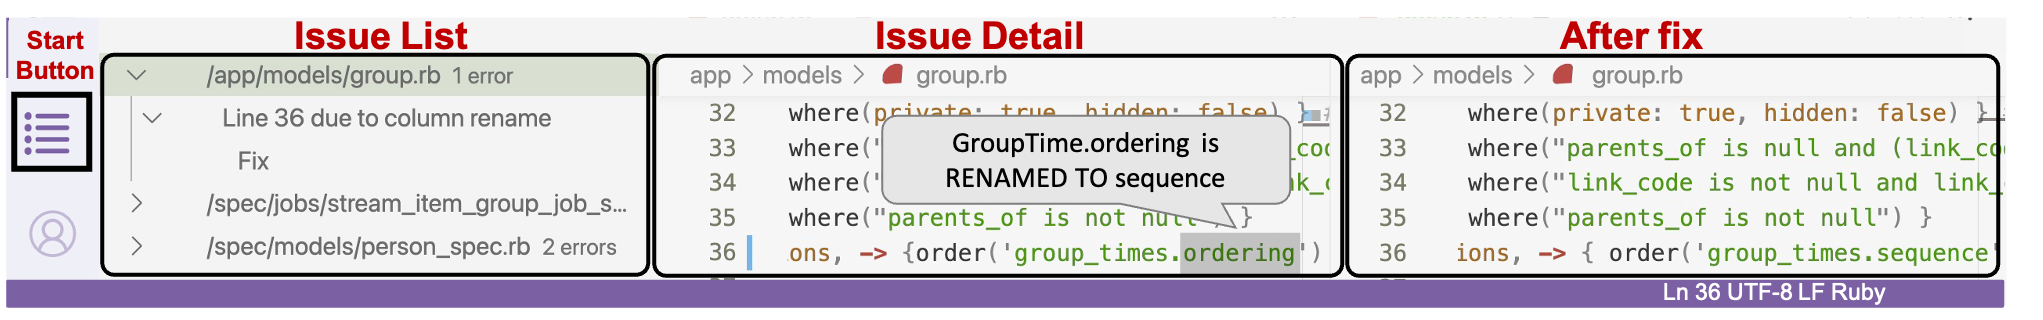
\includegraphics[width=\textwidth]{figs/plugin.png}
\caption{The screenshot of \Tool{} IDE Plugin}
\label{fig:vscode-plugin}
\end{figure*}


We have implemented \Tool{} as a plugin for Visual Studio Code~\cite{vscode}, a popular IDE for multiple languages.
% \shan{citation needed to back this claim up}
As shown in Figure~\ref{fig:vscode-plugin}, one can press the start button to start the plugin. By default, \Tool compares the current code with the latest commit.
% \shan{can I specify which commit to compare against? 
%If this is not difficult to implement, it would be nice to have}. 
Users can also specify the commits they desire to check in the configuration file. 

\textbf{Issue list.} The left panel, as shown in Figure~\ref{fig:vscode-plugin}, lists all the errors detected by \Tool in a hierarchical view. The first level lists
the files where errors are detected; clicking a file shows the details of every 
error in that file, including the line number and the type of root-cause schema change;
clicking the error shows a ``Fix'' button. 

\textbf{Issue detail.} Clicking a file in the issue list will navigate users to the corresponding file in the editor, with the error code highlighted. Users can hover their mouses over the highlighted code and see the detailed
explanation, like ``GroupTime.ordering is RENAMED TO sequence'' in Figure~\ref{fig:vscode-plugin}. 

\textbf{Issues fix.} One can click the  `\texttt{Fix}'  button  on the left panel
or a `\texttt{Fix all}' button to fix one or all the issues.


\subsection{Implementation}
The start button triggers our static analyzer to run on the given
code commits. The analyzer produces an \texttt{output.json} file that is parsed 
%by \texttt{getDepsInPackageJson} 
to create the issue list using  the Visual Studio Code Extension APIs \texttt{TreeDataProvider} and \texttt{TreeItem}. 
The \texttt{DocumentHighlightProvider} API is used to highlight the selected error code, given the filename and line number information in 
\texttt{output.json}. The \texttt{HoverProvider} API enables the tooltip of detailed reason to  display once hovering over the highlighted code.
To fix the error, \texttt{TextDocument}, \texttt{Range}, and  \texttt{ExtensionContext} APIs are used to insert, replace, and delete source code in the editor panel.



